% Qualitative reconstruction of the printed function graph on (0,3).
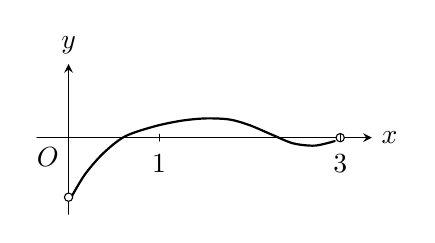
\begin{tikzpicture}[x=1.15cm,y=.72cm,>=stealth,line cap=round,line join=round]
  \draw[->] (-.35,0)--(3.35,0) node[right] {$x$};
  \draw[->] (0,-1.35)--(0,1.3) node[above] {$y$};
  \draw[thick] plot[smooth] coordinates {(.03,-1.05) (.18,-.65) (.38,-.28) (.62,.02) (.95,.20) (1.25,.30) (1.52,.34) (1.78,.32) (2,.22) (2.25,.05) (2.48,-.10) (2.72,-.14) (2.94,-.06)};
  \draw[fill=white] (0,-1.05) circle (1.5pt);
  \draw[fill=white] (3,0) circle (1.5pt);
  \draw (1,-.06)--(1,.06) node[below=4pt] {$1$};
  \draw (3,-.06)--(3,.06) node[below=4pt] {$3$};
  \node[below left] at (0,0) {$O$};
\end{tikzpicture}
